% Important: The shell-escape flag is required for the Minted package.
% Please compile this document with 'pdflatex -shell-escape main.tex'.
% If you are using another IDE, you may be able to specify this in the
% options or to provide an option like '% !TEX option = -shell-escape'
% in this file, depending on your builder. See the README.md for more.

% Don't put any content in here.
% Don't even include content files by using \input or \inlcude.
% Put your content into components/text.tex or include it there using \input.
% You probably want to modify the following files:
%   components/info.tex             contains the author, title etc.
%   components/settings.tex         contains the packages and settings.
%   components/commands.tex         contains helpful custom commands.
%   components/glossary.tex         contains an explanation of the used terms.
%   components/acknowledgements.tex contains the acknowledgements.
%   components/quote.tex            contains a quote.
%   components/abstract.tex         contains the abstract of the document.
%   components/text.tex             includes the actual content of the document.
%   components/outline.tex          contains the outline.
%   components/preface.tex          contains the preface.
%   chapters/                       contains the main text.
%   bibliography/literature.bib     contains the BibTeX entries.
%   images/                         contains all your content-related images.
%
% You probably don't need to change anything in the following files:
%   components/cover.tex            formats the front cover of the document.
%   components/titlepage.tex        formats the title page of the document.
%   components/disclaimer.tex       formats the disclaimer page.
%   styles/                         contains style elements (e.g. logos).
%   main.tex                        contains the top-level code structure.
%   README.md                       contains information about this template.

\documentclass[11pt,
              a4paper,
              index=totoc,
              headsepline,
              footsepline,
              BCOR=12mm,
              DIV=13]{scrbook}

% KOMA scrbook options:
%  index=totoc: include an entry for the index in the table of contents.
%  headsepline: use horizontal line under heading.
%  footsepline: use horizontal line above footer.
%  BCOR: binding correction (e.g.: BCOR=12mm)
%  DIV: Number of sheet sections (used for layout) (e.g.: DIV=13)

% !TEX root = ../main.tex
% Set here the title, authors and other stuff to be used for the cover
% This file is used by MAIN.TEX

% set title, authors and stuff for the cover
\def\university{Technische Universit{\"a}t M{\"u}nchen}
\def\universityLogo{styles/tum_logo}
\def\program{Computational Science and Engineering \\(International Master's Program)}
\def\programLogo{styles/cse_logo}
\def\doctype{Master's Thesis}

\def\title{Small Sparse Matrix Multiplication Kernels for Knights Landing}
\def\author{Nathan W. Brei}
\def\examinerOne{Univ.-Prof.\ Dr.\ Michael Bader}
\def\examinerTwo{Univ.-Prof.\ Dr.\ Thomas Huckle}
\def\assistantAdvisor{Dr.\ rer.\ nat.\ Carsten Uphoff}
\def\date{February 15, 2018}

\def\keywords{{keyword1}, {keyword2}, {keyword3}}

% The following are used for the PDF metadata, by default the same as above.
\def\metaTitle{\title}
\def\metaAuthor{\author}
\def\metaSubject{\doctype\ -\ \university}
\def\metaKeywords{\keywords}

% text to appear in the footer
\def\footertext{}


% !TEX root = ../main.tex
% Included by MAIN.TEX

%--------------------------------------------------
% Fonts and page setup
%--------------------------------------------------

% Default font
%\usepackage{palatino}

% Enable special PostScript fonts (optional)
% \usepackage{pifont}

% Manipulate the footer
\usepackage{scrpage2}
\usepackage{scrhack}
\pagestyle{scrheadings}
\ifoot[\footertext]{\footertext} % \footertext set in INFO.TEX

% Set the font for the section headings
\renewcommand{\sectfont}{\normalfont \bfseries \sffamily}

% Conditional commands in LaTeX documents, used for the \clearemptydoublepage.
\usepackage{ifthen}

% Typeset text in multiple columns (optional)
% \usepackage{multicol}

% Rotation tools, including rotated full-page floats (optional)
\usepackage{rotating}


%--------------------------------------------------
% Document structure
%--------------------------------------------------

% Create glossaries and lists of acronyms
\usepackage[toc, xindy]{glossaries}

% Standard LaTeX package for creating indexes
\usepackage{makeidx}


%--------------------------------------------------
% Bibliography
%--------------------------------------------------

% Set the bibliography style (default: plain)
\bibliographystyle{plain}

% Special biblography package (nice to have)
% \usepackage{natbib}


%--------------------------------------------------
% Graphics and floats
%--------------------------------------------------

% Enhanced support for graphics (recommended)
\usepackage{graphicx}
% Path to the figures directory (default: {figures/})
% Multiple entries are allowed, e.g. {{figures1/}{figures2/}}.
\graphicspath{{figures/}}

% Improved interface for floating objects (optional)
\usepackage{float}

% To use the subfigures (optional)
\usepackage{subcaption}


%--------------------------------------------------
% Mathematics
%--------------------------------------------------

% AMS mathematical facilities for LaTeX (recommended)
\usepackage{amsmath}

% TeX fonts from the American Mathematical Society (recommended)
\usepackage{amsfonts}

% Some extra math symbols (optional)
% \usepackage{amssymb}

% Extended maths fonts for LaTeX (optional)
% \usepackage{yhmath}

% Provide math delimiters whose size can be computed automatically (optional)
% \usepackage{commath}


%--------------------------------------------------
% Source code and algorithms
%--------------------------------------------------

% Source code typesetting
% \usepackage{listings} % (optional - alternative)
\usepackage[newfloat,outputdir=../build]{minted} % (recommended)
% Set global Minted options
\setminted{linenos, autogobble, frame=lines, framesep=2mm}
% Inline C++ (optional)
\newcommand{\incpp}[1]{\mintinline{c++}{#1}}
\newenvironment{code}{\captionsetup{type=listing}}{}
\SetupFloatingEnvironment{listing}{name=Source Code}

% Typeset algorithms - pseudocode (optional)
% \usepackage{algorithmicx}
% \usepackage{algpseudocode}
% Normal arrow comments
% \algrenewcommand{\algorithmiccomment}[1]{\hfill$\rightarrow$ #1}


%--------------------------------------------------
% Tables
%--------------------------------------------------

% Tables (optional)
\usepackage{tabu}

% Add color to LaTeX tables (optional)
% \usepackage{colortbl}

% Create tabular cells spanning multiple rows (optional)
% \usepackage{multirow}


%--------------------------------------------------
% Color
%--------------------------------------------------

% Use colors
\usepackage[dvipsnames]{xcolor}

% You may find all the pre-defined colors in
% https://en.wikibooks.org/wiki/LaTeX/Colors#Predefined_colors

% Custom colors
\definecolor{Pantone300C}{HTML}{0065BD} % TUM primary blue
\definecolor{Pantone301}{HTML}{005293}  % TUM secondary light blue
\definecolor{Pantone540}{HTML}{003359}  % TUM secondary dark blue
\definecolor{DarkGray}{HTML}{333333}    % TUM secondary dark gray
\definecolor{MediumGray}{HTML}{808080}  % TUM secondary medium gray
\definecolor{LightGray}{HTML}{CCCCC6}   % TUM secondary light gray
\definecolor{Pantone7527}{HTML}{DAD7CB} % TUM accent gray
\definecolor{Pantone158}{HTML}{E37222}  % TUM accent orange
\definecolor{Pantone383}{HTML}{A2AD00}  % TUM accent green
\definecolor{Pantone283}{HTML}{98C6EA}  % TUM accent very light blue
\definecolor{Pantone542}{HTML}{64A0C8}  % TUM accent light blue

% Color for the hyperlinks (e.g. table of contents)
\def\colorLinks{Pantone300C}
% Color for the web links
\def\colorUrl{Pantone542}
% Color for the citations
\def\colorCitations{Pantone158}

%--------------------------------------------------
% PDF output
%--------------------------------------------------

% Pro­duce hy­per­text links in the doc­u­ment (recommended)
\usepackage{hyperref}

% Adjust the color of the links
\hypersetup{
  linkcolor=\colorLinks,%
  urlcolor=\colorUrl,%
  citecolor=\colorCitations
}

% Disable the coloring of the links when printing.
% Requires a compatible PDF reader.
\usepackage[ocgcolorlinks]{ocgx2}[2017/03/30]

% PDF Metadata
\hypersetup{
  pdftitle={\metaTitle},%
  pdfauthor={\metaAuthor},%
  pdfkeywords={\metaKeywords},%
  pdfsubject={\metaSubject}
}

% Create XMP Metadata (uses the values from hyperref)
\usepackage{hyperxmp}

% Make thumbnails (optional)
% \usepackage{thumbpdf}


%--------------------------------------------------
% Other settings
%--------------------------------------------------

% Define commands that appear not to eat spaces (optional)
\usepackage{xspace}
\usepackage{tikz}



% !TEX root = ../main.tex
% Included by MAIN.TEX
% Please include your own cool commands here.
% Be only sure to comment it sufficiently so others can use it.

%-------------------------------------------------------------
%                      Own Commands
%-------------------------------------------------------------


%-------------------------------------------------------------
% math stuff -------------------------------------------------

% nice R, N, C
\newcommand{\nat}{\mathbb{N}}
\newcommand{\real}{\mathbb{R}}
\newcommand{\compl}{\mathbb{C}}

% norm
%\newcommand{\norm}[1]{\left\| #1 \right\|}

% un demi
\newcommand{\half}{\frac{1}{2}}

% parantheses
\newcommand{\parenth}[1]{ \left( #1 \right) }
\newcommand{\bracket}[1]{ \left[ #1 \right] }
\newcommand{\accolade}[1]{ \left\{ #1 \right\} }
%\newcommand{\angle}[1]{ \left\langle  #1 \right\rangle }

% partial derivative: %#1 function, #2 which variable
% simple / single line version
\newcommand{\pardevS}[2]{ \delta_{#1} f(#2) }

% fraction version
\newcommand{\pardevF}[2]{ \frac{\partial #1}{\partial #2} }

% render vectors: 3 and 4 dimensional
\newcommand{\veciii}[3]{\left[ \begin{array}[h]{c} #1 \\ #2 \\ #3	\end{array} \right]}
\newcommand{\veciv}[4]{\left[ \begin{array}[h]{c} #1 \\ #2 \\ #3 \\ #4	\end{array} \right]}

% render matrices: 3  dimensional (arguments in row first order)
\newcommand{\matiii}[9]{\left[ \begin{array}[h]{ccc} #1 & #2 & #3 \\ #4 & #5 & #6 \\ #7 & #8 & #9	\end{array} \right]}


%-------------------------------------------------------------
%-------------------------------------------------------------


%-------------------------------------------------------------
% some abreviations ------------------------------------------
\newcommand{\Reg}{$^{\textregistered}$}
\newcommand{\reg}{$^{\textregistered}$ }
\newcommand{\Tm}{\texttrademark}
\newcommand{\tm}{\texttrademark~}
\newcommand {\bsl} {$\backslash$}

%-------------------------------------------------------------
%-------------------------------------------------------------


%-------------------------------------------------------------
% formating --------------------------------------------------

% Theorem & Co environments and counters
\newtheorem{theorem}{Theorem}[chapter]
\newtheorem{lemma}[theorem]{Lemma}
\newtheorem{corollary}[theorem]{Corollary}
\newtheorem{remark}[theorem]{Remark}
\newtheorem{definition}[theorem]{Definition}
\newtheorem{equat}[theorem]{Equation}
\newtheorem{example}[theorem]{Example}
%\newtheorem{algorithm}[theorem]{Algorithm}

% inserting figures
\newcommand{\insertfigure}[4]{ % Filename, Caption, Label, Width percent of textwidth
	\begin{figure}[htbp]
		\begin{center}
			\includegraphics[width=#4\textwidth]{#1}
		\end{center}
		\vspace{-0.4cm}
		\caption{#2}
		\label{#3}
	\end{figure}
}

% referecing figures

\newcommand{\refFigure}[1]{ %label
	figure \ref{#1}
}
\newcommand{\refChapter}[1]{ %label
	chapter \ref{#1}
}

\newcommand{\refSection}[1]{ %label
	section \ref{#1}
}

\newcommand{\refParagraph}[1]{ %label
	paragraph \ref{#1}
}

\newcommand{\refEquation}[1]{ %label
	equation \ref{#1}
}

\newcommand{\refTable}[1]{ %label
	table \ref{#1}
}

\newcommand{\rigidTransform}[2]
{
	${}^{#2}\!\mathbf{H}_{#1}$
}

% comment that appears on the border - very practical !!!
\newcommand{\comment}[1]{\marginpar{\raggedright \noindent \footnotesize {\textsl{#1}} }}

% page clearing
\newcommand{\clearemptydoublepage}{%
  \ifthenelse{\boolean{@twoside}}{\newpage{\pagestyle{empty}\cleardoublepage}}%
  {\clearpage}}

%-------------------------------------------------------------
%-------------------------------------------------------------

\newcommand{\etAl}{\emph{et al.}\mbox{ }}


% !TEX root = ../main.tex
\newglossaryentry{computer}
{
  name=computer,
  description={is a programmable machine that receives input,
               stores and manipulates data, and provides
               output in a useful format}
}

\newglossaryentry{poc}
{
  name={proof of concept},
  description={}
  }
\newglossaryentry{ui}
{
  name={user interface},
  description={}
  }
\newglossaryentry{ai}
{
  name={arithmetic intensity},
  description={a measure of floating-point operations (FLOPs)
              \hyphenation{per-formed} performed by a \hyphenation{gi-ven} given code or code section relative
              to the amount of memory accesses (Bytes) that are required
               to support those operations\cite{AI}}
  }

\newglossaryentry{speed-up}
{
  name={speed-up},
  description={the factor of temporal acceleration a program
  exhibits when additional computational resources are dedicated to it's execution.}
}

\newglossaryentry{directive pragmas}
{
  name={directive pragma},
  description={a computer programming language construct that specifies how a compiler
  should process input data} % sourced from wikipedia
}


\newglossaryentry{rc}{%SOURCE: wikipedia
name={race condition},
description={A race condition or race hazard is the behavior of an electronic,
 software, or other system where the output is dependent on the sequence or
 timing of other uncontrollable events. It becomes a bug when events do not
 happen in the order the programmer intended. The term originates with the idea
 of two signals racing each other to influence the output first.}
}
\newglossaryentry{dd}{
name={data dependencies},
description={}
}
\newglossaryentry{sisd}{
name={single instruction single data},
description={}
}
\newglossaryentry{simt}{
name={single instruction multiple threads},
description={}
}

\newglossaryentry{simd}{
name={single instruction multiple data},
description={}
}
\newglossaryentry{gp}{%SOURCE: wikipedia
name={Gaussian Plane},
description={The two dimensional plane of complex numbers.}
}
\newglossaryentry{CURAND}{
name={CURAND},
description={
The CURAND library provides facilities that focus on the simple and efficient
generation of high-quality pseudorandom and quasirandom numbers.\cite{cuRAND}
}
}

\newacronym[longplural={partial differential equations}]{PDE}{PDE}{partial differential equations}
\newacronym{mpi}{MPI}{Message Passing Interface}

\newacronym[longplural={Random Walks on Spheres}]{RWoS}{RWoS}{Random Walk on Spheres}

\newacronym[longplural={graphical processing units}]{GPU}{GPU}{graphical processing unit}

\newacronym[longplural={central processing units}]{CPU}{CPU}{central processing unit}
\newacronym{hpc}{HPC}{high performance computing}

\newacronym[longplural={arithmetic logic units}]{ALU}{ALU}{arithmetic logic unit}

\newacronym[longplural={streaming multi-processors}]{SM}{SM}{streaming multi-processor}

\newacronym[longplural={boundary value problems}]{BVP}{BVP}{boundary value problem}
\newacronym[longplural={general purpose graphical processing units}]{GPGPU}{GPGPU}{general purpose graphical processing units}
\newacronym{CUDA}{CUDA}{compute unified device architecture}
\newacronym{RAM}{RAM}{random access memory}
\newacronym{SRAM}{SRAM}{static random access memory}
\newacronym{DRAM}{DRAM}{dynamic random access memory}
\newacronym{I/O}{I/O}{input/output}
\newacronym{PTX}{PTX}{Parallel Thread eXecution}
\newacronym{jit}{JIT}{just in time}


\newacronym[longplural={floating point operations}]{FLOP}{FLOP}{floating point operation}
\newacronym[longplural={abstract syntax trees}]{AST}{AST}{abstract syntax tree}
\newacronym[longplural={general matrix multiplications}]{GEMM}{GEMM}{general matrix multiplication}
\newacronym[longplural={fused multiply adds}]{FMA}{FMA}{fused multiply add}
\newacronym[longplural={vector processing units}]{VPU}{VPU}{vector processing unit}
\newacronym[longplural={domain specific languages}]{DSL}{DSL}{domain specific language}


\newacronym{KNL}{KNL}{knights landing}
\newacronym{CSC}{CSC}{compressed sparse column}
\newacronym{CSR}{CSR}{compressed sparse row}
\newacronym{BSC}{BSC}{block sparse column}
\newacronym{BSR}{BSR}{block sparse row}
\newacronym{BCSC}{BCSC}{block compressed sparse column}
\newacronym{BCSR}{BCSR}{block compressed sparse row}
\newacronym{VBCSC}{VBCSC}{virtual block compressed sparse column}
\newacronym{VBCSR}{VBCSR}{virtual block compressed sparse row}










\makeglossary

\begin{document}

 \frontmatter

 % !TEX root = ../main.tex
% The front cover.
% Included by MAIN.TEX

%--------------------------------------------------
% The Front Cover
%--------------------------------------------------

% correct BCOR - undo at the end !!!
\def\bcorcor{0.15cm}
\addtolength{\hoffset}{\bcorcor}

\thispagestyle{empty}

\vspace{4cm}
\begin{center}
	\includegraphics[width=4cm]{\universityLogo}\\
	\vspace{5mm}
	\huge \program \\
	\vspace{0.5cm}
	\large \university
\end{center}

\vspace{20mm}
\begin{center}
	{\Large \doctype}\\
	\vspace{20mm}
	{\huge \textbf \title}\\
	\vspace{15mm}
	{\LARGE  \author}\\
	\vspace{\fill}
	\includegraphics[width=4cm]{\programLogo}
\end{center}


 \clearemptydoublepage

 % !TEX root = ../main.tex
% The titlepage.
% Included by MAIN.TEX


%--------------------------------------------------
% The title page
%--------------------------------------------------

% correct BCOR - undo at the end !!!
\def\bcorcor{0.15cm}
\addtolength{\hoffset}{\bcorcor}

\thispagestyle{empty}

\vspace{4cm}
\begin{center}
    \includegraphics[width=4cm]{\universityLogo}\\
    \vspace{5mm}
    \huge \program \\
    \vspace{0.5cm}
    \large \university
\end{center}

\vspace{10mm}
\begin{center}
    {\Large \doctype}\\
    \vspace{10mm}
    {\LARGE \title}\\
    \vspace{10mm}

    \begin{tabular}{ll}
      \Large Author:                        & \Large \author \\[2mm]
      \Large 1\textsuperscript{st} examiner:& \Large \examinerOne\\[2mm]
      \Large 2\textsuperscript{nd} examiner:& \Large \examinerTwo \\[2mm]
      \Large Assistant advisor:             & \Large \assistantAdvisor \\[2mm]
      \Large Submission Date:               & \Large \date
    \end{tabular}

    \vspace{\fill}
    \includegraphics[width=4cm]{\programLogo}
\end{center}

% undo BCOR correction
\addtolength{\hoffset}{\bcorcor}


 % !TEX root = ../main.tex
\clearemptydoublepage

\thispagestyle{empty}
\vspace*{0.7\textheight}
\noindent
I hereby declare that this thesis is entirely the result of my own work except where otherwise indicated. I have only used the resources given in the list of references.

\vspace{15mm}
\noindent
\date \hspace{5cm} \author
\newpage


 % !TEX root = ../main.tex
\clearemptydoublepage
\phantomsection
\addcontentsline{toc}{chapter}{Acknowledgements}

\vspace*{2cm}

\begin{center}
{\Large \textbf Acknowledgments}
\end{center}

\vspace{1cm}

\begin{center}
I would like to thank:

\begin{itemize}
\item My family
\item My advisor, Carsten Uphoff.
\item Roland?
\item Natasha?
\item The TUM chair of scientific computing for providing me access to their KNL cluster
\end{itemize}

\end{center}


 \clearpage
\phantomsection

\begin{center}
\vspace*{9cm}
\textit{"Science is what we understand well enough to explain to a computer.}

\textit{Art is everything else we do."}
\end{center}
\par
\hspace*{7cm}
\textit{-Donald Knuth}


 % !TEX root = ../main.tex
% The abstract.
% Included by MAIN.TEX

\clearemptydoublepage
\phantomsection
\addcontentsline{toc}{chapter}{Abstract}

\vspace*{2cm}
\begin{center}
{\Large \textbf Abstract}
\end{center}
\vspace{1cm}

This document will serve as an example to you, of how to use \LaTeX to write your
CSE Master's Thesis. It will have examples and recomendations, and hopefully a
few laughs.  Because this is the abstract, it will have to convince you that this 
template is something you want to use.  It has been proven, that without using
this template, writing your thesis will be much more dificult. The template is
based on previous work, and has been improved apon and updated.  The result of 
this template is a modern latex template that everyone can contribute to and use
for their studies of CSE @ TUM.

Some more great abstract tips can be found here: 
\href{https://users.ece.cmu.edu/~koopman/essays/abstract.html}{Great Abstract tips}


 \tableofcontents

 \mainmatter

 \addtolength{\evensidemargin}{-12mm}

 % !TEX root = ../main.tex
\chapter{Introduction}
\label{chapter:Introduction}


\section{Motivation}

A worthwhile use of the vast computational resources available in 2018 is on seismic simulations. 

\begin{description}
	\item[SeisSol]
    Simulates earthquakes, specifically, dynamic rupture processes and seismic wave propagation over an unstructured tetrahedral mesh. 

    \item[ADER-DG]
    A numerical method which uses Discontinuous Galerkin discretization in space and ADER discretization in time. It avoids a global system matrix, using local element matrix operations instead.

    \item[Small Sparse Matrix Multiplications]
    The compute kernels resemble the operation shown below, applied recursively. Different sparsity patterns are used, but they are all known at compile time.
\end{description}

\begin{figure}
  \centering
  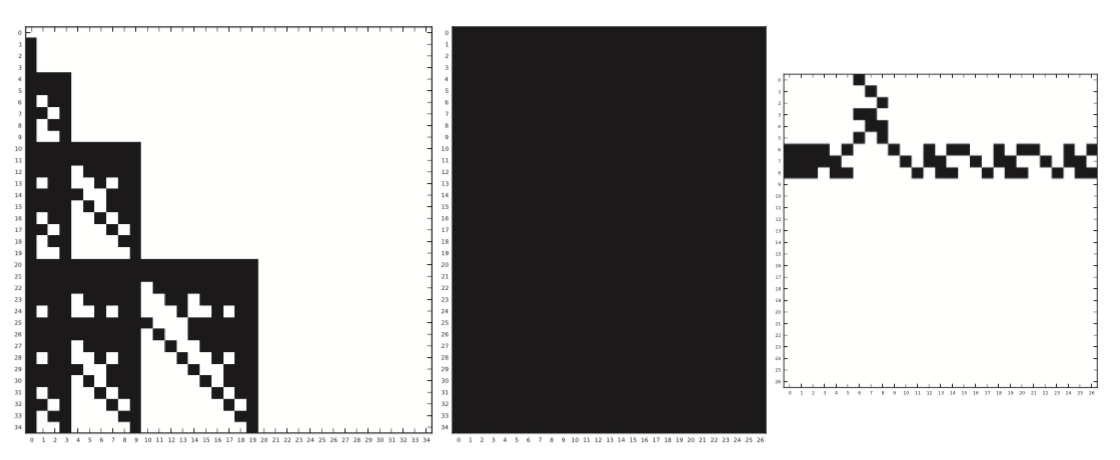
\includegraphics[height=3cm]{images/seissol_visc.png}
  \caption{Common sparsity patterns in SeisSol}
  \label{fig:seissol_star}
\end{figure}

\section{Hardware Constraints}
\label{section:knl}

Although the motivation is straightforward, it is growing increasingly difficult to implement in practice because it is working against current trends in computer architecture. An growing number of the top500 computers are using GPUs or Xeon Phis. This trend is likely to continue because it allows greater parallelism at a lower energy cost. It was desired to run the code on LRZ's CoolMUC3 cluster, which uses Knights Landing.

Knights Landing (KNL) is the second-generation Intel Xeon Phi, a manycore processor that offers greater parallelism and less power consumption in exchange for a slower clock speed. An overview is given by~\cite{Sodani:2016:KLS:2927511.2927563} and a more comprehensive resource is given by~\cite{Jeffers:2016:IXP:3050856}. Unlike its predecessor, Knights Corner, KNL is a host processor rather than a coprocessor, which means that it can run the entire x86-64 instruction set, albeit with a performance penalty for some operations. KNL has two kinds of memory, a high-bandwidth MCDRAM and a high-capacity DDR4. Each processor contains between 64 and 72 cores with 4 hyperthreads per core, resulting in at least 256 logical CPUs. The instruction-level parallelism is similarly impressive, being the first processor to implement the AVX-512 instruction set extensions. These provide 32 vector registers, each of which holds 64 bytes, allowing 8 double-precision floating point numbers to be operated on simultaneously in each \gls{VPU}. Instruction-level performance is further improved by an enhanced \gls{FMA} instruction, which performs $c := c + a*b$ in a single cycle, optionally including a broadcast and a mask. Thus the theoretical peak performance of each chip is given as:

\[
36~\frac{tiles}{chip} \times 2~\frac{cores}{tile} \times 2~\frac{VPUs}{core} \times 16~\frac{double~flops}{VPU \cdot cycle} \times 1.3~\frac{GCycles}{sec} = 3~\frac{double~TFlop}{sec\cdot chip}
  \label{eq:knl_peak_perf}
\]

This peak performance is in practice merely an upper bound, as it assumes a steady-state throughput of 2 FMAs per cycle. The only algorithms which come close to achieving this are dense matrix multiplication and (to a lesser extent) LU and Cholesky factorization. If the algorithm cannot be vectorized at all, the attainable performance drops by a factor of 8, and if it cannot use the FMA instructions, it drops by a further factor of 2. Hence inherently scalar algorithms perform dramatically worse. This may be a reasonable tradeoff: since scalar algorithms are much more likely to be memory-bound, the extra flops might be wasted. Nevertheless this provides a strong incentive to find creative ways to make the most of the vector registers. 

Another key constraint is cache bandwidth. With only one store unit, KNL can store at most 64B/cycle, corresponding to one vector register. This means that it is essential to accumulate all possible changes to that vector register before storing it. It also makes loop unrolling more important, since this is the only way to amortize the cost of loads and stores.

A number of related bottlenecks encompass the instruction pipeline. Because Knights Landing was derived from the older Silvermont architecture, which was optimized for low power consumption, the instruction pipeline is simpler and narrower. The instruction cache can only provide 16B/cycle, and the decoder can only handle 2 instructions/cycle. Meanwhile, a single \gls{FMA} instruction takes up between 7 and 10 bytes. The most important constraint, however, is that the out-of-order execution pipeline can only issue 2 instructions per cycle. This means that any instruction which is not an FMA \emph{displaces} an FMA, halving the potential computational efficiency of one cycle.


\begin{figure}[tb]
\centering
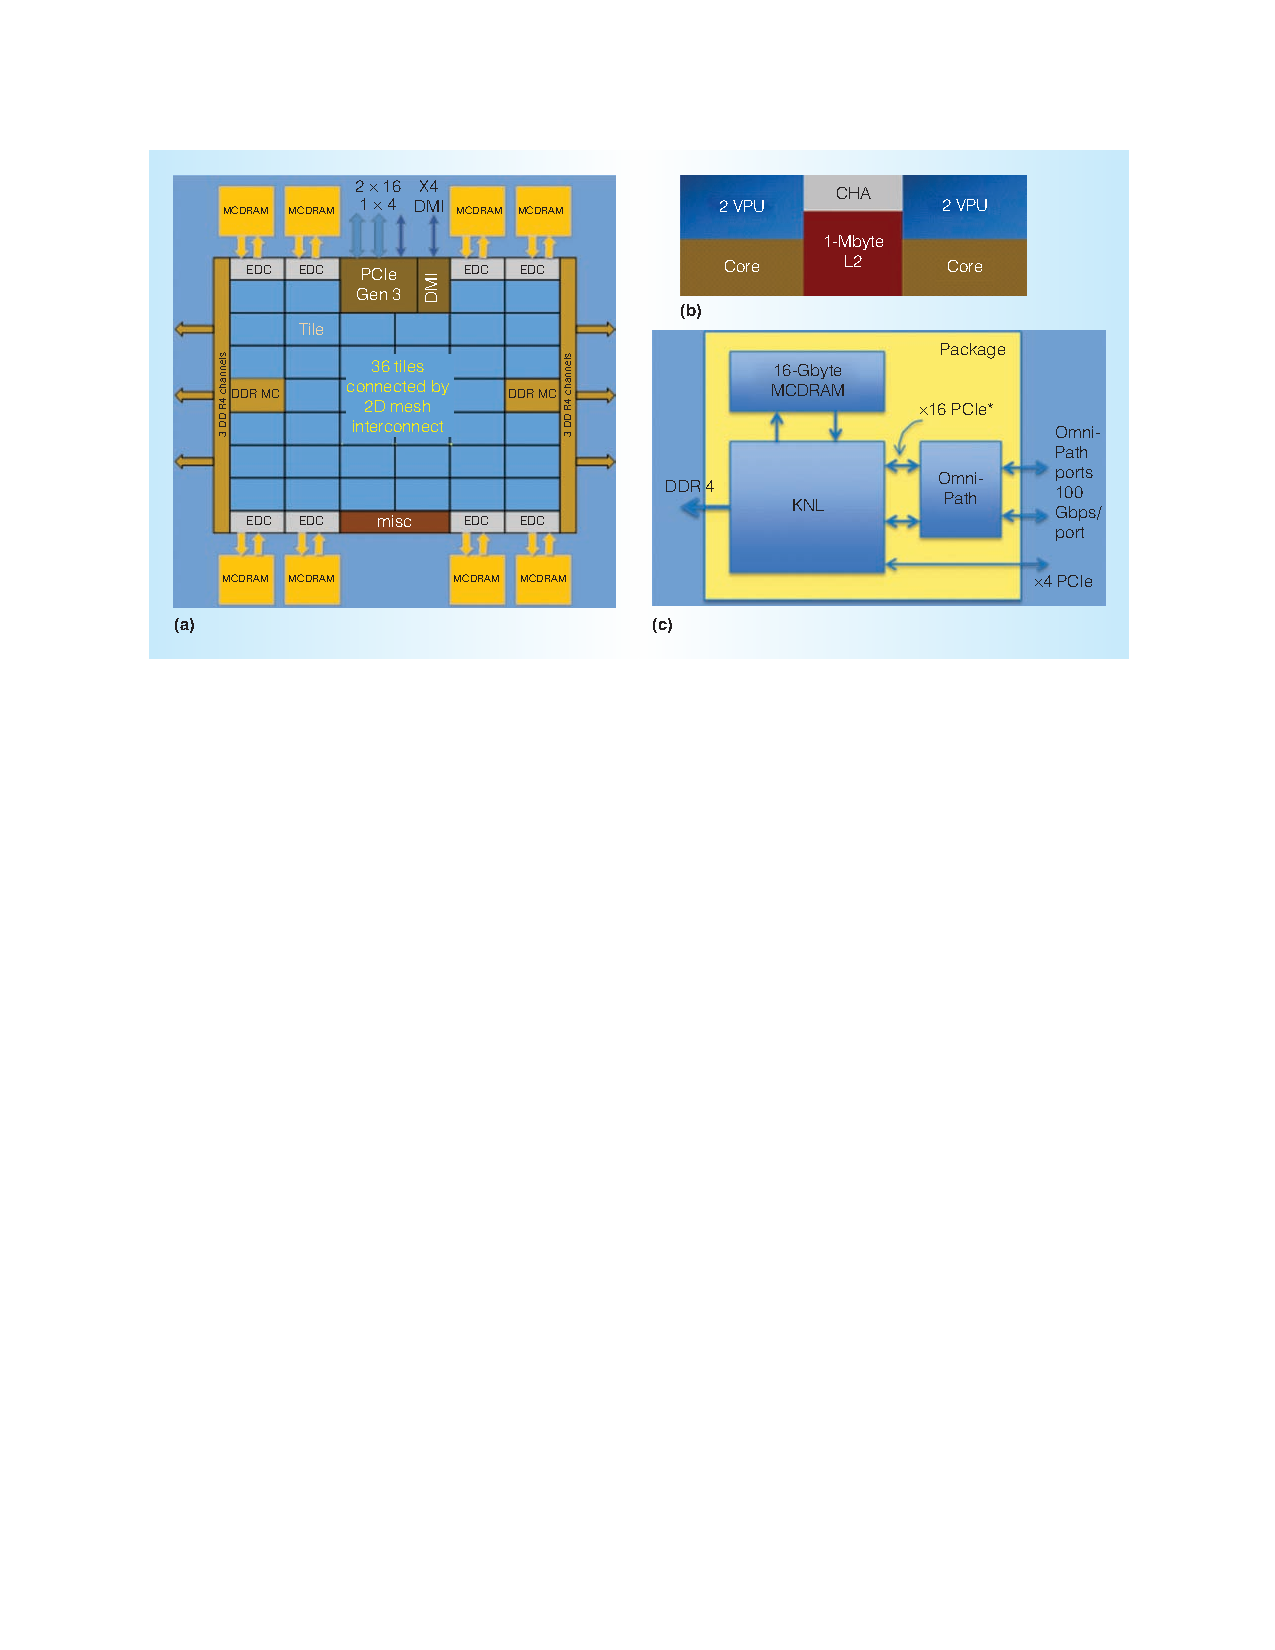
\includegraphics[width=\textwidth]{images/knl_arch.pdf}
\caption{Block diagram of the Knights Landing architecture, taken from~\cite{Sodani:2016:KLS:2927511.2927563}. As shown in (a), each processor is divided into 36 tiles connected in a 2D mesh. As shown in (b), each tile contains 2 cores and a shared L2 cache. Each core has two VPUs and its own L1 caches.}
\end{figure}

\section{Previous approaches}

There is already a substantial amount of effort invested in improving the compute kernels of SeisSol. 

\subsection{CSC sparse multiplication}
  The first approach used standard compressed-sparse-column multiplication. This algorithm goes back to WHOM? . It looks as follows:


  It has the following advantages: It is extremely general, placing no constraints on the matrix size or sparsity. 
  The sparsity pattern itself is known only at runtime. This generality makes it extremely amenable to abstraction, so a 

  Nevertheless, the standard csc multiplication algorithm suffers from several crucial disadvantages: 

\begin{description}
  \item[High memory usage]

  \item[Computational intensity]

  \item[Inability to unroll the innermost loop] This hurts pipeline efficiency.

  \item[Scalar operations]

  The indices are looked up at runtime. Firstly, this requires storing the indices, doubling the amount of memory needed. If only one matrix is sparse, the total number of flops is $2 * m * n * nnz$, with nnz=1/4*n*k, this means that the arithmetic intensity [FLOPs/byte] is 1/8 that of dense matrix multiplication. 
  Although the format lays everything out in memory as efficiently, the algorithm must nevertheless loop over k. The resulting control dependency prevents . The fact that the sparsity pattern is only known at compile time prevents unrolling. 
  A dense-by-sparse algorithm would still benefit from vectorization, but if the 

\end{description}


In the case of SeisSol, the sparsity patterns are derived from the basis functions, which themselves depend mainly on order of accuracy and the choice of viscous damping model. These parameters are all chosen at compile time. Secondly, the problem size is always small: the largest dimension is either 34 (corresponding to ) 56. 

In the case of Knights Landing, these problems are all acerbated. 


  Standard compressed-sparse-column multiplication
    \begin{itemize}
      \item[$+$] Generality.
      \item[$+$] Algorithm uses a (small) constant number of instructions.
      \item[$-$] Index lookups require indirect memory access, causing lots of problems for the execution pipeline.
      \item[$-$] $sparse \times sparse$ is fundamentally scalar. (However, BSR can be vectorized.)
      \item[$-$] Disregards the fact that the sparsity pattern is known at compile time.
    \end{itemize}

  Sparsity pattern unrolled into instruction stream
    \begin{itemize}
    \item[$+$] Index lookups removed completely
    \item[$+$] $dense \times sparse$ case can be vectorized perfectly 
    \item[$-$] Generates one FMA instruction for every nonzero
    \item[$-$] (Implementation) Memory access pattern is suboptimal on KNL
    \item[$-$] (Implementation) Intel compiler struggles to generate efficient assembly
    \end{itemize}

  Current approach: Dense matrix multiplication via libxsmm
    \begin{itemize}
    \item[$+$] Memory access patterns and register blockings optimized for KNL
    \item[$+$] (Implementation) Code generator emits assembly directly 
    \item[$-$] Filling in zero entries wastes both flops and memory bandwidth
    \end{itemize}


  \section{Goals, approach, and design space}

  Each of the existing algorithms discussed in the preceding section encounter different  bottlenecks and constraints. \py{SpGemm} and \py{libxsmm} solve a more general problem than strictly necessary, and Breuer does not use registers Thus there appears to be room to create more complicated algorithms which combine the desirable features of each. The three existing algorithms can be thought of as poles in a barycentric design space, and the aim is to find points in the middle which finesse around the bottlenecks in the corners. One corner has high compute intensity and optimal register usage but wasted flops; another has no wasted flops but many control dependencies and lower compute intensity; the last has no wasted flops and high compute intensity, but poor register usage. The center ought to have decent compute intensity, decent register usage, few control dependencies, and few wasted flops. 


  To keep the scope of this work bounded, we adhere to following assumptions:
  \begin{itemize}
    \item The sparse matrix has a fixed pattern which is known at compile time.
    \item The memory layout of the sparse matrix is not constrained elsewhere.
    \item All matrices fit in the L2 cache: $(mn + mk + kn)\cdot 8 \leq 1e6$
  \end{itemize}

  Within this framework, we consider variations of the following:
  \begin{itemize}
    \item Modifications of the sparsity pattern
    \item Modifications of the control flow
    \item The memory layout of the sparse matrix
    \item The block sizes, if a block decomposition is used
    \item The ordering and unrolling of the loop nest
  \end{itemize}


Although interesting, we disregard prefetching, instruction alignment, and register assignment. 

The goal of this work is to find algorithms which might outperform the status quo, and write a code generator which will emit an instance of each relevant algorithm for a given problem. The generator should be able to handle different matrix sizes, number of nonzeros, and sparsity patterns, while staying within the aforementioned assumptions. 

Once implemented, the generators can be tested -- using the actual SeisSol matrices -- to determine if they yield a speedup. Equally interesting is exploring the algorithm's problem space constraints. Using both the observed and estimated performance, we can address the questions ``which problems can this algorithm handle efficiently?'' and ``which algorithm is best for a given problem?''. 

Each algorithm requires additional tuning parameters, and the effect of these should also be estimated and tested, addressing the question ``which parameters yield the best kernel for a given problem?''. If possible, heuristics should be given in order to choose these parameters automatically.

   
\section{Roadmap} 
  This work is broken down as follows. Chapter 2 lays out the fundamental concepts and terminology. Chapter 3 covers a progression of different dense-by-sparse kernels in depth, and discusses strategies for sparse-by-dense and tensor kernels which might benefit from a similar treatment. Chapter 4 discusses the design of the code generator, and provides a brief manual illustrating its use. Chapter 5 walks through some experiment results, attempting to discern performance and scaling characteristics. Finally, Chapter 6 wraps everything up.











 \chapter{Background}
\label{chapter:review}

\section{Matrix multiplication}

Dense and sparse matrix multiplication account for a surprising fraction of all computation, particularly in scientific and engineering fields. Since any optimization or algorithmic improvement has the potential to improve the performance of programs across the board, these algorithms have been organized under a series of common interfaces. Not only does this make it easy to reuse the best known implementation of many fundamental linear algebra operations, but it also confers other advantages: robustness is increased by the careful handling of edge cases, portability is increased because a programmer can link to the best implementation for their target architecture, and readability is increased because numerical algorithms can all work at the same abstraction level. The first such interface, \gls{BLAS}, was introduced in 1979 by Lawson~\cite{Lawson:1979:BLA:355841.355847} and only supported dense vector and matrix operations. Later interfaces, such as LAPACK, build upon and extend \gls{BLAS} to support increasingly complex operations; the history and design of such interfaces is covered by Dongarra in~\cite{Dongarra:1998:NLA:552704}. 

Most of the naming conventions used in this work follow those of BLAS and its successors. The arguments for each operation get quite complicated (see~\cite{IntelCSCMM}), but for our purposes they can be simplified as shown in Figure~\ref{fig:blas}. These conventions have propagated to libraries including MKL and libxsmm.

\begin{figure}
\begin{verbatim}
// C = alpha*A*B + beta*C
dgemm(m, n, k, alpha, A, lda, B, ldb, beta, C, ldc)
\end{verbatim}

\begin{tabular}{ll}
	\toprule
	Variable    &  Meaning \\
	\midrule
	dgemm & Double General Matrix Multiplication \\
	alpha & A scalar constant \\
	beta  & A scalar constant \\
	A     & A matrix of doubles, in dense column-major format unless sparse \\
	B     & A matrix of doubles, in dense column-major format unless sparse \\
	C     & A matrix of doubles, in dense column-major format \\
	m     & The number of rows of C and A \\
	n     & The number of columns of C and B \\
	k     & The number of columns in A and rows in B \\
	lda   & The leading dimension (offset between columns) of A; zero indicates sparse \\
	ldb   & The leading dimension (offset between columns) of B; zero indicates sparse \\
	ldc   & The leading dimension (offset between columns) of C \\


	\bottomrule
\end{tabular}
\caption{Simplified BLAS naming conventions for general matrix multiplication}
\label{fig:blas}
\end{figure}


A sparse BLAS interface was not standardized until 2002, as described by Duff in~\cite{Duff:2002:OSB:567806.567810}. Compared with the dense case, sparse matrix operations are considerably more difficult to pin down because the performance of each operation depends heavily -- often asymptotically -- on the memory layout, which in turn depends on both the chosen storage format and the sparsity pattern, which is often known only at runtime. The choice of storage format is tightly coupled with the implementation of the operations, making abstraction difficult. Thus there are a multitude of different storage formats, with not entirely consistent naming conventions. The formats used in this work are described in Figure~\ref{fig:formats} and illustrated throughout Chapter~\ref{chapter:algs}. Ultimately, a sparse BLAS works well when the matrices are large, are constrained to a common format such as CSC, and have unpredictable or nonconstant sparsity patterns; otherwise a custom implementation might be able to do much better.

\begin{figure}

\begin{description}
	\item[Dense (DNS)] Column-major dense format, possibly padded
	\item[Coordinate format (COO)] 
	\item[Compressed sparse column (CSC)] Nonzero entries are stored column-by-column left to right. 
	\item[Compressed sparse row (CSR)]
	\item[Block sparse column (BSC)]
	\item[Block sparse row (BSR)]
	\item[Block compressed sparse column (BCSC)]
	\item[Block compressed sparse row (BCSR)]
	\item[Diagonal (DIA)]
	\item[Virtual... (V...)] Any sparse format where the index information has been omitted.
\end{description}


\caption{Descriptions of different sparse matrix formats as used in this work. Naming conventions vary between literature; pay attention to the distinction between BSC and BCSC. }
\label{fig:formats}
\end{figure}

What did Goto figure out?

However, it wasn't until 2008 that a more general approach for designing optimized dense matrix multiplication algorithms -- independent of the exact details of the memory hierarchy -- was established. This work by Goto takes advantage of the recursive nature of block-wise matrix multiplication in order to successively divide the problem into blocks, each of which is sized and padded to make best use of the memory hierarchy. Thus a very large matrix may be split among separate machines using Cannon's algorithm, then further split into blocks which fit in the L2 cache, then in the L1 cache, then finally in the registers themselves. 

Goto's work , GotoBLAS, influenced BLIS. 


Why doesn't Goto's work apply here?

What is the outer-product formulation?

What does Libxsmm do differently from BLAS/Goto?

What about memory-addressing schemes

What about Breuer's work? Does it vectorize?

What is the sparse/dense asymmetry?

What naming conventions do we use?



\section{Variable naming conventions}


This work uses the BLAS naming conventions wherever possible. These conventions must be extended to handle 
Firstly, iteration variable names are derived from the size variable names by adding the suffix \py{-i}. Secondly, we wish to iterate not only over cells, but also blocks and vectors. The naming convention handles this via a prefix. In effect, \py{m,n,k} determine the iteration \emph{direction}, and the prefix determines the units. Finally, we introduce the direction \py{l} to handle the third dimension, when working with tensors. The complete grammar is provided in Figure~\ref{fig:grammar}. This convention adds much-needed predictability and ease of comprehension inside deeply nested loops. It also helps ensure that iteration variables stay within the correct range. The most common pattern is to iterate over matrix blocks, and then inside each block iterate over cells (for sparse matrices) and vectors (for dense matrices). An example of this is given below:

\begin{minted}{python}
for ki in range(k):
	print(B[ki,ni])
\end{minted}

\begin{figure}[tbh]
  \centering
  \begin{subfigure}[l]{0.48\textwidth}
      \begin{minted}[linenos=false,fontsize=\small]{text}
    <var>       ::= [<units>]<direction>[i]
    <units>     ::= b | B | v | V
    <direction> ::= m | n | k | l
  \end{minted}
  \end{subfigure}
  ~~~~
  \begin{subfigure}[r]{0.45\textwidth}
    \centering
    \begin{tabular}{cll}
		\toprule
		Units    & Mnemonic & Meaning \\
		\midrule

		none  & Cell          & Cells in the matrix      \\
		b     & Intra-block   & Cells in a block         \\
		B     & Inter-block   & Blocks in the matrix     \\
		v     & Intra-vector  & Cells in a block         \\
		V     & Inter-vector  & Vectors in a block       \\
		\bottomrule
	\end{tabular}
  \end{subfigure}
  \caption{Grammar for variable names.}
  \label{fig:grammar}
\end{figure}


\section{The outer-product formulation}

Having subdivided a large matrix into blocks small enough to fit in registers, and having chosen the optimal traversal order for these blocks, it only remains to perform the multiplication of these blocks themselves. This is not trivial due to the constraints of working with vector registers. The state of the art is known as the outer-product formulation.

\begin{figure}[ht]
\begin{minted}[fontsize=\footnotesize]{gas}
# Load C register block
vmovapd 0(%rdx),  %zmm16                                 # load C[:,0]
vmovapd 64(%rdx), %zmm17                                 # load C[:,1]
vmovapd 128(%rdx), %zmm18                                # load C[:,2]
# ...

# Load A register block
vmovapd 0(%rdi), %zmm0                                   # load A[:,0]
vmovapd 64(%rdi), %zmm1                                  # load A[:,1]
# ...

# Outer product of A[:,0] * B[0,:]
vfmadd231pd 0(%rsi) {1to8}, %zmm0, %zmm16                # C[:,0] += A[:,0] .* B[0,0]
vfmadd231pd 0(%rsi,%r15,1) {1to8}, %zmm0, %zmm17         # C[:,1] += A[:,0] .* B[0,1]
vfmadd231pd 0(%rsi,%r15,2) {1to8}, %zmm0, %zmm18         # C[:,2] += A[:,0] .* B[0,2]
# ...

# Outer product of A[:,1] * B[1,:]
vfmadd231pd 8(%rsi) {1to8}, %zmm1, %zmm16                # C[:,0] += A[:,1] .* B[1,0]
vfmadd231pd 8(%rsi,%r15,1) {1to8}, %zmm1, %zmm17         # C[:,0] += A[:,1] .* B[1,1]
vfmadd231pd 8(%rsi,%r15,2) {1to8}, %zmm1, %zmm18         # C[:,0] += A[:,1] .* B[1,2]
# ...
# More outer products ...

# Store C register block
vmovapd %zmm16, 0(%rdx)                                  # store C[:,0]
vmovapd %zmm17, 64(%rdx)                                 # store C[:,1]
vmovapd %zmm18, 128(%rdx)                                # store C[:,2]
# ...
\end{minted}
\caption{Example outer-product formulation generated by libxsmm}
\label{fig:outerproduct}
\end{figure}

\section{Sparsity pattern unrolling}

\section{Memory addressing schemes}

The simplest scheme is to use pointer-offset addressing, where the pointer is in a register and the offset is hardcoded, such as \texttt{rsi + 22}. The downside of this approach is that when the offset is greater than 128*8, (i.e. there are more than 128 nonzeros in B), the resulting FMA instructions take up 10 bytes, which will cause a bottleneck as described in Section~\ref{section:knl}. A more sophisticated scheme uses scale-index addressing, which uses two registers and two hardcoded values, such as \texttt{B + 8*i + 22}. These FMA instructions only take up 7 bytes; their main downside is that the generated code becomes harder to understand.




\section{Dense-by-sparse vs sparse-by-dense asymmetry}
(Dense $\times$ Sparse) $\neq$ (Sparse $\times$ Dense) due to vectorization

Choice of row-major vs column-major format determines which of the two vectorizes nicely: $(AB)^T = B^T A^T$

- Outer-product formulation
- Breuer
- MKL
- Row-major vs Column-major


 \chapter{Dense-by-Sparse Algorithms}
\label{chapter:algs}

The main focus of this thesis is on improving the performance of small dense-by-sparse matrix multiplication algorithms. It is necessary to finesse around the bottlenecks that constrain the approaches described in the previous chapter. The extra information which makes this possible is the sparsity pattern known at compile time. Figure~\ref{fig:dxsp} shows the different algorithms under consideration and the relationship between them. The starting point is the outer-product formulation generated from \texttt{libxsmm}. This forms the basis of SparseMicrokernel. 

There exist well-established conventions for naming variables inside matrix multiplication algorithms. 
The use of the letters m,n,k is unavoidable. However, the conventions become less clear when the loops are nested over blocks, vectors, and cells.
Another point of confusion is naming iteration variables. This work adopts the following naming conventions:

  \begin{minted}[fontsize=\footnotesize]{text} 
    <var>       ::= [<units>] <dimension> [i]
    <units>     ::= b | B | v | V
    <dimension> ::= m | n | k | l
  \end{minted}

The units indicates what is being counted or iterated over:

    \begin{tabular}{cll}
\toprule
Units    & Mnemonic & Meaning \\
\midrule

none  & Cell          & Cells in the matrix      \\
b     & Intra-block   & Cells in a block         \\
B     & Inter-block   & Blocks in the matrix     \\
v     & Intra-vector  & Cells in a block         \\
V     & Inter-vector  & Vectors in a block       \\
\bottomrule
\end{tabular}

The dimension indicates 

\begin{tabular}{cl}
\toprule
Dimension    & Meaning \\
\midrule
m & Rows of A and C \\
n & Columns of B and C \\
k & Columns of A, rows of B \\
l & The third dimension of A and C\\
\bottomrule
\end{tabular}


Finally, 'i' indicates that this is an iteration variable.
For example, one may confidently assume that the variable $bni \in [0, bn-1]$ iterates cell-by-cell across columns of B and C within the current block.



\begin{figure}[H]
  \centering
  

\usetikzlibrary{shapes,arrows}
\usetikzlibrary{decorations.pathreplacing}


% Define block styles
\tikzstyle{decision} = [diamond, draw, fill=blue!20, 
    text width=4.5em, text badly centered, node distance=3cm, inner sep=0pt]

\tikzstyle{block} = [rectangle, draw, fill=gray!20, 
    text width=7em, text centered, minimum height=3em]

\tikzstyle{line} = [draw, -latex']

\tikzstyle{cloud} = [draw, ellipse,fill=red!20, node distance=3cm,
    minimum height=2em]

\begin{tikzpicture}[node distance = 5em, auto]
    % Place nodes

    \node [block] (microkernel) {Sparse\\ microkernel};
    \node [block, left of=microkernel, node distance=10em] (libxsmm) {Libxsmm dense outer product};
    \node [block, below of=microkernel] (macrokernel) {Fully unrolled\\ sparse};
    \node [block, below of=macrokernel] (tiledsparse) {Tiled sparse};
    \node [block, right of=tiledsparse, node distance=10em] (blocksparse) {Block sparse};
    \node [block, below of=tiledsparse] (paddedsparse) {Padded sparse};
    \node [block, below of=blocksparse] (generalsparse) {General sparse};
    \node [block, below of=paddedsparse] (paddeddiagsparse) {Padded sparse with extracted diagonal};

    %\node [block, left of=evaluate, node distance=3cm] (update) {update model};
    %\node [decision, below of=evaluate] (decide) {is best candidate better?};
    %\node [block, below of=decide, node distance=3cm] (stop) {stop};

    % Draw edges
    \path [line] (libxsmm) -- (microkernel);
    \path [line] (microkernel) -- (macrokernel);
    \path [line] (macrokernel) -- (tiledsparse);
    \path [line] (tiledsparse) -- (blocksparse);
    \path [line] (tiledsparse) -- (paddedsparse);
    \path [line] (paddedsparse) -- (generalsparse);
    \path [line] (blocksparse) -- (generalsparse);
    \path [line] (paddedsparse) -- (paddeddiagsparse);

    \draw [decorate,decoration={brace,amplitude=10pt},xshift=0pt,yshift=0pt]
(1.75,-2) -- (4.75,-2)node [black,midway,yshift=9pt] {\footnotesize Irregular block offset};

    \draw [decorate,decoration={brace,amplitude=10pt},xshift=0pt,yshift=0pt]
(-2,-7.25) -- (-2,-4.25) node [black,midway,xshift=-8pt,text width=5em] {\footnotesize Multiple\\ Microkernels};
    %\path [line] (evaluate) -- (decide);
    %\path [line] (decide) -| node [near start] {yes} (update);
    %\path [line] (update) |- (identify);
    %\path [line] (decide) -- node {no}(stop);
    %\path [line,dashed] (expert) -- (init);
    %\path [line,dashed] (system) -- (init);
    %\path [line,dashed] (system) |- (evaluate);
\end{tikzpicture}



  \label{fig:dxspfamilies}
  \caption{Relationships between different dense-by-sparse multiplication algorithms}
\end{figure}





\section{Sparse Microkernel}

The SparseMicrokernel is our first attempt to account for the sparsity pattern while building off of the state of the art for dense matrix multiplication. Our key assumption is that the matrices A and C are small enough to fit entirely in registers: $(n + k) * (m/8) <= 32$. Generating the dense GEMM for this problem effectively extracts the dense microkernel. This microkernel has no loops (otherwise it couldn't amortize the cost of loading and storing A and C) and this makes it easy to modify.

The sparse microkernel is a straightforward modification of the dense microkernel. All FMA instructions \texttt{C[:,ni] += A[:,ki] .* B[ki, ni]} where \texttt{B[ki, ni] = 0} due to the sparsity pattern are removed. This is tricky to do in a general way; an abstraction designed for the purpose is described at length in Section X.XX. Next, any loads of a column of A corresponding to an empty row of B are removed. Finally, any loads and stores of a column of C corresponding to an empty column of B are removed. This last step is often not desirable, as shall be discussed later, so the option is controlled by a parameter.

Now we consider the format of the sparse matrix B. Keeping B dense is suboptimal because the algorithm will be streaming adjacent nonzeros and it would be helpful if they occupied the same cache line. Breuer and Heinecke used a \emph{virtual} compressed sparse column format, where the nonzeros were laid out in a plain 1D array ordered by columns. For SparseMicrokernel, a virtual compressed row format might yield the best locality, but this is insignificant because few cache lines are involved on sparse matrices of this size. Having chosen the format, the next step is to choose an addressing scheme for the elements of the sparse matrix. The simplest scheme is to use pointer-offset addressing, where the pointer is in a register and the offset is hardcoded, such as \texttt{rsi + 22}. The downside of this approach is that when the offset is greater than 128*8, (i.e. there are more than 128 nonzeros in B), the resulting FMA instructions take up 10 bytes, which will cause a bottleneck as described in section X.XX. A more sophisticated scheme uses scale-index addressing, which uses two registers and two hardcoded values, such as \texttt{B + 8*i + 22}. These FMA instructions only take up 7 bytes; their main downside is that the generated code becomes harder to understand.

Another question is alignment. The alignment of B is not particularly important because its elements are loaded one at a time, but very important for A and C, which are loaded in a vectorwise fashion. If not aligned on a 64-byte boundary, the vector load operation will suffer a delay because the data is split across two cache lines. Using the aligned vector load operation \texttt{vmovapd} will trigger a segmentation fault if the pointer is not actually aligned. On the other hand, the unaligned version \texttt{vmovupd} can handle both the aligned and unaligned case, and will not incur the penalty if the pointer is in fact aligned. 

The performance of SparseMicrokernel shall be explored in Section X.XX. It is clear that removing the FMA instructions decreases the arithmetic intensity, and if the nonzeros are evenly distributed, there will be no accompanying decrease in memory bandwidth. Nevertheless the algorithm remains compute-bound and hence experiences an improved time-to-solution compared to its dense counterpart. Regardless of performance, SparseMicrokernel has limited utility in real problems, since it can only be applied to extremely small matrices. It is valuable primarily as a building block for the more complex algorithms developed next.

* What does the pseudocode look like?

\begin{itemize}
    \item Assume a dense A and a sparse B, with a fixed pattern known at compile time. As discussed in Section X.XX, 
    \item Pack B into a virtual compressed-sparse-row or column format
    \item Remove all fused-multiply-add and load instructions which are not needed
    \item Make this the basic building block for more complicated algorithms 
\end{itemize}




However, this has the following limitations:
\begin{itemize}
    \item Sparsity pattern must be known at compile time
    \item Pattern must fit within vector registers: $m \leq 8;  n \leq 30$
    \item (Dense $\times$ Sparse) $\neq$ (Sparse $\times$ Dense) due to vectorization
    \item Choice of row-major vs column-major format determines which of the two vectorizes nicely: $(AB)^T = B^T A^T$
\end{itemize}




The SparseMicrokernel algorithm is a straightforward modification: FMA instructions which operate on 
broadcasted zero entries are eliminated, and the memory addresses of the nonzero entries are 
shifted so that a sparse matrix format with better memory locality can be used. If an entire 
row of B is zero, the corresponding column of A is not needed, so the corresponding load 
operation is removed. Traversing the sparse matrix, finding the nonzeros, and finding the correct
memory address for each cell is done using a high-level cursor abstraction, as described elsewhere.   

Eliminating the unnecessary instructions reduces both computational intensity and memory traffic.


\begin{figure}[ht]
      \begin{minted}[fontsize=\footnotesize]{text}
        {text}
        loop over m blocks:

           unroll loop over n blocks:

              load C block into registers

              unroll loop over k blocks:

                 load A block into registers
                 microkernel for current B block
                 move A right 1 block
                 move B down 1 block

              store C block from registers
              move A to far left
              move B to top + right 1 block
              move C right 1 block

           move A down 1 block
           move C down 1 block
      \end{minted}
\end{figure}


\section{Unrolled dense-by-sparse multiplication}

Generate sparse microkernels for each (k,n) block of B, and unroll these into the instruction stream.
\begin{itemize}
      \item[$+$] Supports arbitrary matrix sizes
      \item[$+$] Dense-style register blocking for a dense $\times$ sparse algorithm.
      \item[$+$] Does not fill in any zeros -- no wasted flops

      \item[$-$] Generates an FMA instruction for each nonzero
      \item[$-$] These FMA instructions are 10B, too large to stream
      \item[$-$] Irregular location of blocks in memory prevents using tricks to reduce instruction size
      \item[$-$] Total number of nonzeros is limited by size of instruction cache.

\end{itemize}

\begin{figure}[tb]
  \centering
  \begin{subfigure}[b]{0.32\textwidth}
    \centering
          \[
      \left[
          \begin{array}{c c c | c c c }
          0 &   &   & 10 &   &   \\
          1 & 2 &   & 11& 12&   \\
            & 3 & 4 &   & 13& 14  \\
          \hline
          5 &   &   & 15  &   &   \\
          6 & 7 &   & 16  &17   &   \\
            & 8 & 9 &   & 18  &19   \\
          \end{array}
          \right]
      \]
    \caption{TiledSparse}
    \label{fig:tiledblocks}
  \end{subfigure}
  \begin{subfigure}[b]{0.32\textwidth}
    \centering
      \[
      \left[
          \begin{array}{c c c | c c c }
          0 &   &   &    &    &    \\
          1 & 2 &   &    &    &    \\
            & 3 & 4 &    &    &    \\
          \hline
          5 &   &   & 10 &    &    \\
          6 & 7 &   & 11 & 12 &    \\
            & 8 & 9 &    & 13 & 14 \\
          \end{array}
          \right]
      \]    \caption{BlockedSparse}
    \label{fig:blockedblocks}
  \end{subfigure}
    \begin{subfigure}[b]{0.32\textwidth}
    \centering
      \[
      \left[
          \begin{array}{c c c | c c c }
          0 &   &   &    &    &    \\
          1 & 2 &   &    &    &    \\
            & 3 & 4 &    &    &    \\
          \hline
          5  & 6  & 7  &    &  14& 15  \\
          8  & 9  & 10 &    &    & 16 \\
          11 & 12 & 13 &    &    &    \\
          \end{array}
          \right]
      \]    \caption{GeneralSparse}
    \label{fig:generalblocks}
  \end{subfigure}
  \caption{Sample matrices illustrating the blocking constraints for different GEMM algorithms. As shown in~\ref{fig:tiledblocks}, TiledSparse
  admits only a single block pattern which is tiled perfectly over the entire matrix. BlockedSparse admits a single block pattern along with empty blocks. GeneralSparse relaxes further to admit multiple different patterns. The numbers indicate the cell's index when using a block compressed-sparse-row format. }
  \label{fig:matrixblocks}

\end{figure}


\section{Tiled dense-by-sparse multiplication}

     The basic idea behind TiledSparse is to scale the FullyUnrolledSparse algorithm to 
matrices with more than 3100 nonzeros by assuming that the sparsity pattern is perfectly regular. 
Specifically, we assume that there is a single sparsity pattern which tiles over the entire matrix
and can be encoded as either a SparseMicrokernel or a FullyUnrolledSparse. The former, of course,
subjects the tiled sparsity pattern to register block size constraints, whereas the latter merely 
subjects it to number-of-nonzeros constraints. Our tiling assumption can be made without loss 
of generality because we can always fill in zeros until we arrive at a regular pattern. (One
way to do this is to partition the original matrix with a desired blocksize, and then take the 
logical union of the sparsity patterns in each block.) The assumption does result in a loss of 
practicality, however, as often the pattern will degenerate to dense. If the pattern is dense, 
and the pattern-blocksize is chosen sensibly, the resulting algorithm will be very similar to 
libxsmm.

There are several ways in which this algorithm may be modified. The first design variable is the
choice of loops to unroll. Because each pattern-block occupies the same amount of memory, the 
loops need only update the pointer to the current block, and thus may be unrolled trivially. 
The optimal amount of unrolling depends mainly on the number of nonzeros in the sparsity pattern.

The second design variable is the representation of the sparse matrix in memory. The choice will
directly affect both memory locality and FMA instruction size. (As discussed elsewhere, it is 
helpful to keep the pointer's offset under 128, as FMA instructions above that threshold are
10 bytes and below are 7 bytes.) A key constraint is regularity: This algorithm assumes it is
possible to traverse the matrix block-by-block using simple pointer arithmetic, which constrains 
the main layouts to (V){CSR, CSC, BCSR, BCSC}. (This assumption will be relaxed in 
later algorithms.) The layout which best suits the memory accesses made by TiledSparse 
is VBCSR. If the layout is prescribed externally as something other than (V){BCSR, BCSC), 
or if the pattern contains more than 128 nonzeros, it is recommended to use multiple cursors in 
order to keep the FMA instruction size down. One possible interoperability trick is to store 
the matrix in COO format, but order the values according to VBCSR. Of course, this is fragile 
if the matrix gets modified.

As mentioned earlier, the main limitation to this algorithm is the tendency for the block pattern to 
fill in until it becomes mostly dense. Otherwise, it is limited to having fewer than ~3000 nonzeros 
in the pattern. It does not require the tiling to be perfect (where the bottommost and rightmost 
tiles are full sized), although this makes the generator more complicated and reduces the allowed 
number of nonzeros in the pattern to $3000 - nnz(top_right) - nnz(bottom_right) - nnz(bottom_left)$. 



        Assume there exists a sparse pattern which tiles perfectly over B.
        \begin{itemize}
        \item[$+$] We can reuse a single microkernel, reducing the number of instructions
        \item[$+$] We can visit blocks in a loop efficiently, using pointer tricks to reduce instruction size.
        \item[$-$] This regularity assumption is likely too strong.
        \item[$-$] In practice, the sparsity pattern would often become dense.
        \end{itemize}




\section{Block dense-by-sparse multiplication}

  Assume that B is decomposed into blocks which are either empty or `full'. `Full' blocks all have the same sparsity pattern. This is a sparse generalization of the block-sparse-column format.

  \begin{itemize}
  \item[$+$] We can reuse a single microkernel, reducing the number of instructions
  \item[$+$] The zero blocks reduce the number of filled-in nonzeros.
  \item[$-$] We can no longer visit blocks by using a loop with pointer arithmetic. \\Our options are:
    \begin{itemize}
    \item Look up the block location from a table in memory
    \item Unroll the block locations into the instruction stream and repeatedly jump to the microkernel.
    \end{itemize}
  \end{itemize}




* What are the performance bottlenecks?
* What sparse matrix format constraints?
* What block size constraints?
* On which matrices is this likely to be efficient? On which matrices is this likely to be inefficient?


\section{General dense-by-sparse multiplication}

The general dense-by-sparse algorithm comes from relaxing \emph{both} of the TiledSparse constraints: There can be any number of different blocks, and each block may contain any number of nonzeros. GeneralSparse maintains a collection of SparseMicrokernel GEMMs 

This algorithm is subject to the following constraints:

\begin{enumerate}

  \item The total number of indirect jumps must be minimized. This implies that the total number of nonzero blocks should be as small as possible. 

  \item The routine must fit in the 32kB instruction cache, which constrains both the sum of nonzeros in each \emph{unique} block, as well as the total number of nonzero blocks. The latter constraint could possibly be finessed by storing the pointers to the start of each block and the corresponding GEMM routine in an array in the data cache instead of unrolling it into the instruction stream.

  \item The sparse matrix should be stored in \emph{block} compressed sparse row or column format in order to have good data locality.

  \item Blocks should be uniformly sized. This is an implementation detail; the constraint may be removed in the future by implementing another MatrixCursor as described in Section X.XX.

\end{enumerate}


GeneralSparse degrades gracefully, similar to TiledSparse. As the matrices grow larger and denser, satisfying constraints (1) and (2) will lead to the unique blocks merging (and thereby filling in) until the algorithm resembles BlockSparse or TiledSparse. However, the overhead due to the indirect jumps means that BlockSparse or TiledSparse will prove to be more performant choice past a certain size.


How do we automatically choose GeneralSparse parameters?

\section{Extracted diagonal}

One pattern which emerges in sparse matrices is to 
 \chapter{Implementation}
\label{chapter:implementation}

\section{Frontends}
\subsection{sparsemmgen}
\subsection{libxsmmproxy}
\begin{itemize}
	\item Auto-choosing parameters
	\item Hardcoding parameters
\end{itemize}
\subsection{runexperiment}
\begin{itemize}
	\item Running via SLURM
\end{itemize}


\section{Code generation}
\begin{itemize}
	\item Choice of language/patterns
	\item Inspiration from older languages
\end{itemize}

\section{Components}
\subsection{Register blocks}
\subsection{Microkernels}

\section{Cursors}

\section{Symbolic execution and reification}


 
\chapter{Experiments}
\label{chapter:experiments}


\section{Performance comparison of practical examples}

The goal of the first experiment is to show that the general approach can yield a speedup on matrices which are of practical interest. In the case of SeisSol, the compute kernels are recursively nested matrix multiplications of the pattern $Q' \mathrel{{+}{=}} K \cdot Q \cdot A$, where $K$ and $A$ are sparse and $Q$ is dense. The $A$ matrix always has the same shape and sparsity pattern, whereas there are many different matrices shaped like $K$. The performance of various kernels on the $Q \cdot A$ multiplication is depicted in Figure~\ref{fig:perf_seissol}. 

Unfortunately, the case of the $K \cdot Q$ multiplication can not be simply plugged in to SeisSol due to the asymmetry between dense and sparse multiplication discussed in Section X.XX. However, if the dense matrices were stored in row-major format instead of column-major, the situation would be reversed. Because the $K$ matrix is larger, this might yield a greater speedup on SeisSol as a whole. For these reasons the transposed problem $Q \cdot K$ is also considered in Figure~\ref{fig:perf_seissol_K}.


The experimental setup is straightforward. The problem size is set as $m=40,~n=15,~k=9$, corresponding to a viscoelastic rheological model as described in~\cite{7568431}. The sparsity pattern used is shown on the right in Figure~\ref{fig:seissol_star}. The only variable measured is wall clock time, which was used to calculate speedup relative to \py{libxsmm}'s dense kernel. The two new kernels tested are UnrolledSparse and GeneralSparse. The only available degree of freedom for matrices this small is the $m$-block size; the two extremes, $bm=8$ and $bm=40$, were both considered. The TiledSparse and BlockSparse kernels, on the other hand, were not considered because they would either degenerate to UnrolledSparse or produce complete fill-in, depending on the chosen block sizes $bn, bk$. The performance of Breuer's sparse kernels was also tested for comparison. 



  \begin{figure}[!htb]
    \centering
%    \begin{subfigure}[b]{0.4\textwidth}
%      \centering
      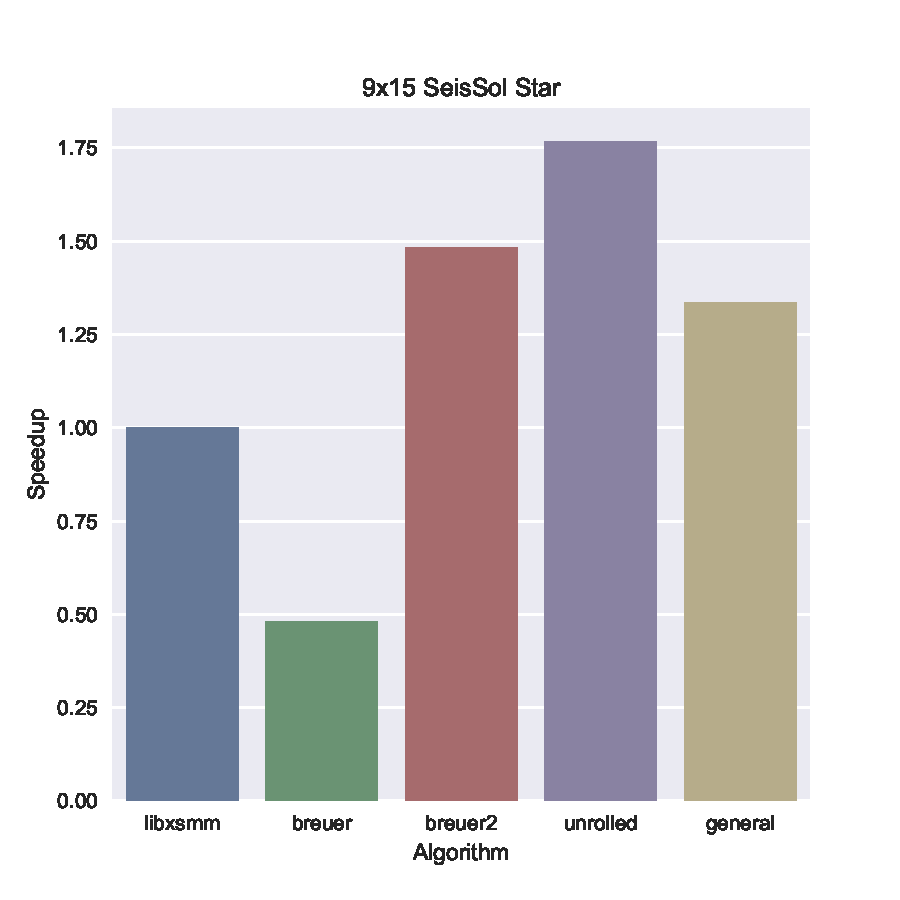
\includegraphics[width=0.75\textwidth]{images/seissol_comparison.pdf}
      \caption{Performance comparison of different spgemm kernels for the 9x15 SeisSol `star' matrix}
      \label{fig:perf_seissol}
%    \end{subfigure}
  \end{figure}


The experiment shows that the UnrolledSparse kernel with $bm=8$ has the best performance, corresponding to a speedup of $1.83$ over dense. To put this in context, the upper bound on the speedup for this problem is $(n\cdot k)/nnz = 3.97$. The UnrolledSparse with the larger block size performs slightly worse, at $1.74$. The GeneralSparse with the larger block size performed similarly worse than its UnrolledSparse equivalent, which was expected due to the indirect jump penalty. Meanwhile, the GeneralSparse with the small block size experienced a slowdown. 

The automatically generated Breuer kernel also experienced a slowdown relative to dense, which was not surprising due to the analysis in Section X.XX. However, an examination of the code revealed a bug: the SIMD vector length was being constrained to 32 bytes instead of 64. Manually fixing this led to a speedup of almost $1.5$ over dense, significantly better but still less than the UnrolledSparse kernel. The performance of the modified Breuer is expected to be similar for small matrices but then diverge as they get larger and denser, due to Breuer's lack of an accumulator for blocks of $C$. 

This experiment can be repeated for different patterns of $K$, and also for the $A$-matrix sizes $n \in \{27, 36\}$. 


\section{Choice of block sizes}

The previous section demonstrated the utility of UnrolledSparse kernel, and also showed that the choice of block sizes $bm,bn,bk$ affects the overall performance. The KNL architecture places a number of constraints on the optimal block size, which is described in depth for the dense case by~\ref{Heinecke:2016:LAS:3014904.3015017}. The goal of this experiment is to test the performance of UnrolledSparse for different block sizes and see to what extent the empirical sparse results match with the theoretical dense analysis. This can also lead to heuristics for automatically choosing the block sizes.

For the experimental setup, we chose $m=n=k=96$ because it has a lot of convenient divisors and it is relatively large. This not only reduces measurement noise, but also stresses the data cache and possibly the instruction cache. Two cases were considered, $nnz=500$ and $nnz=2000$. The sparsity pattern was generated from a uniform random distribution. Kernels were generated for every choice of $bm \in \{8,16,24,32\}$ and $bn, bk \in \{1,2,3,4,6,8,12,16,24\}$ satisfying the MicroSparse constraint $(bk+bn) \cdot (bm/8) \leq 32$. 

The speedups of each kernel relative to dense are shown in Figure~\ref{fig:unrolled_sizing}. Unexpectedly, the plots indicate that the block sizes $bm, bn, bk$ may be chosen with a certain amount of independence. First we consider $bm$. The plots for $bm=24,32$ have been omitted, but they show the same trend: doubling $bm$ decreases the speedup by somewhere between 0.2 and 1, across the board, except in cases where the speedup was already less than 1. This is consistent with libxsmm, which moved from a 2D blocking of C to a 1D blocking specifically for KNL. 

Next we consider $bk$


  \begin{figure}[!htb]
    \centering
    \begin{subfigure}[b]{0.45\textwidth}
      \centering
      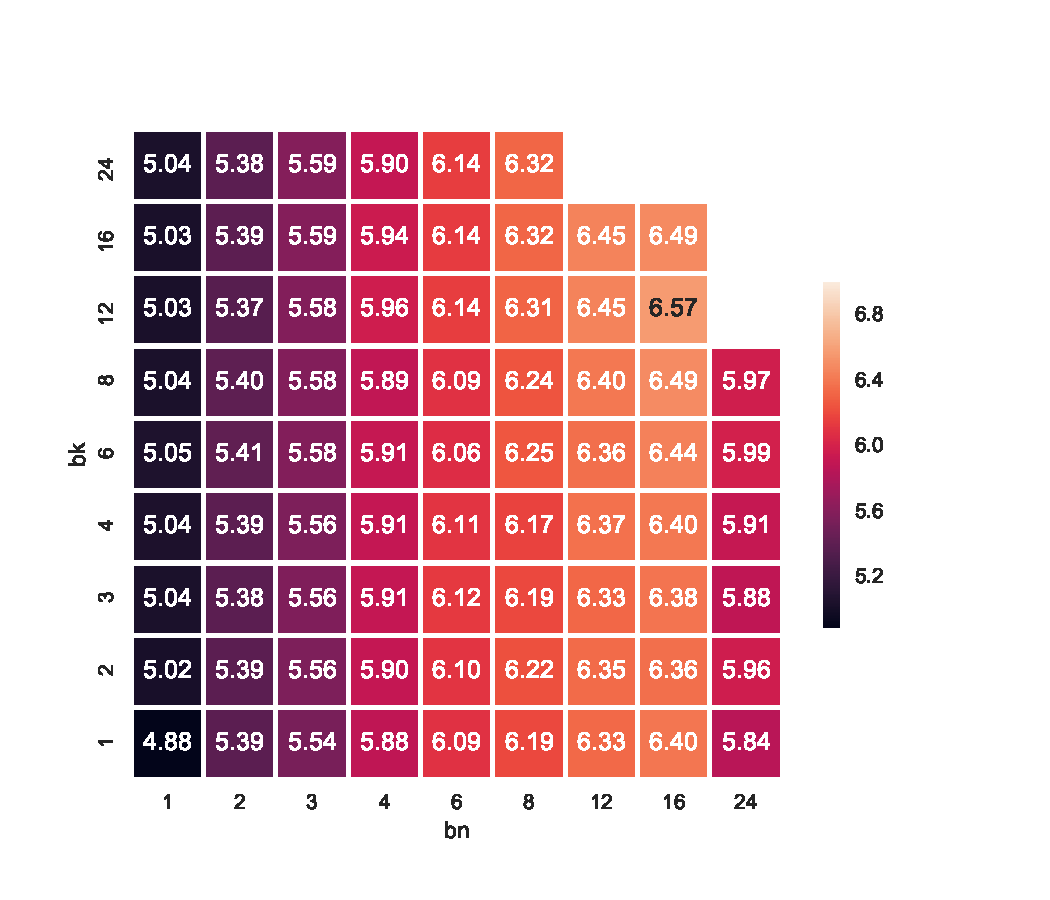
\includegraphics[width=\textwidth]{images/unrolled_sizing_500_8.pdf}
      \caption{bm = 8, nnz = 500}
    \end{subfigure}
    \begin{subfigure}[b]{0.45\textwidth}
      \centering
      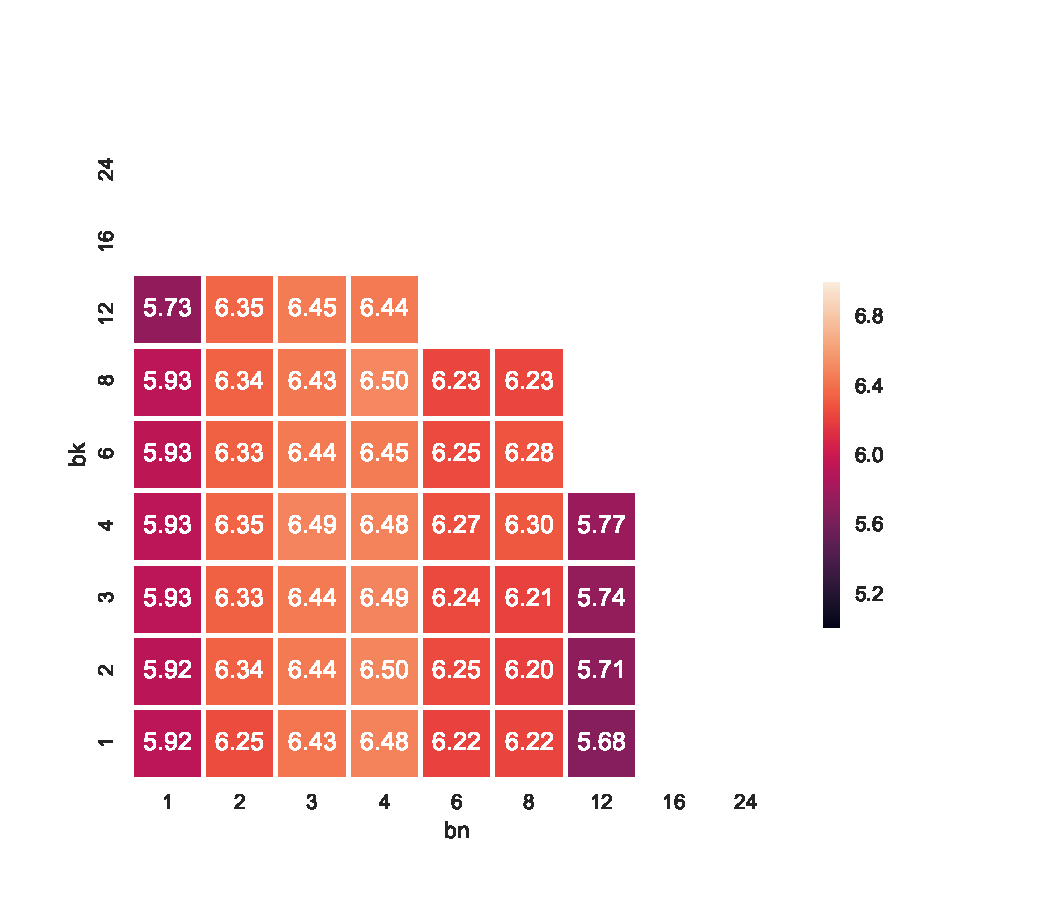
\includegraphics[width=\textwidth]{images/unrolled_sizing_500_16.pdf}
      \caption{bm = 16, nnz = 500}
    \end{subfigure}
    \begin{subfigure}[b]{0.45\textwidth}
      \centering
      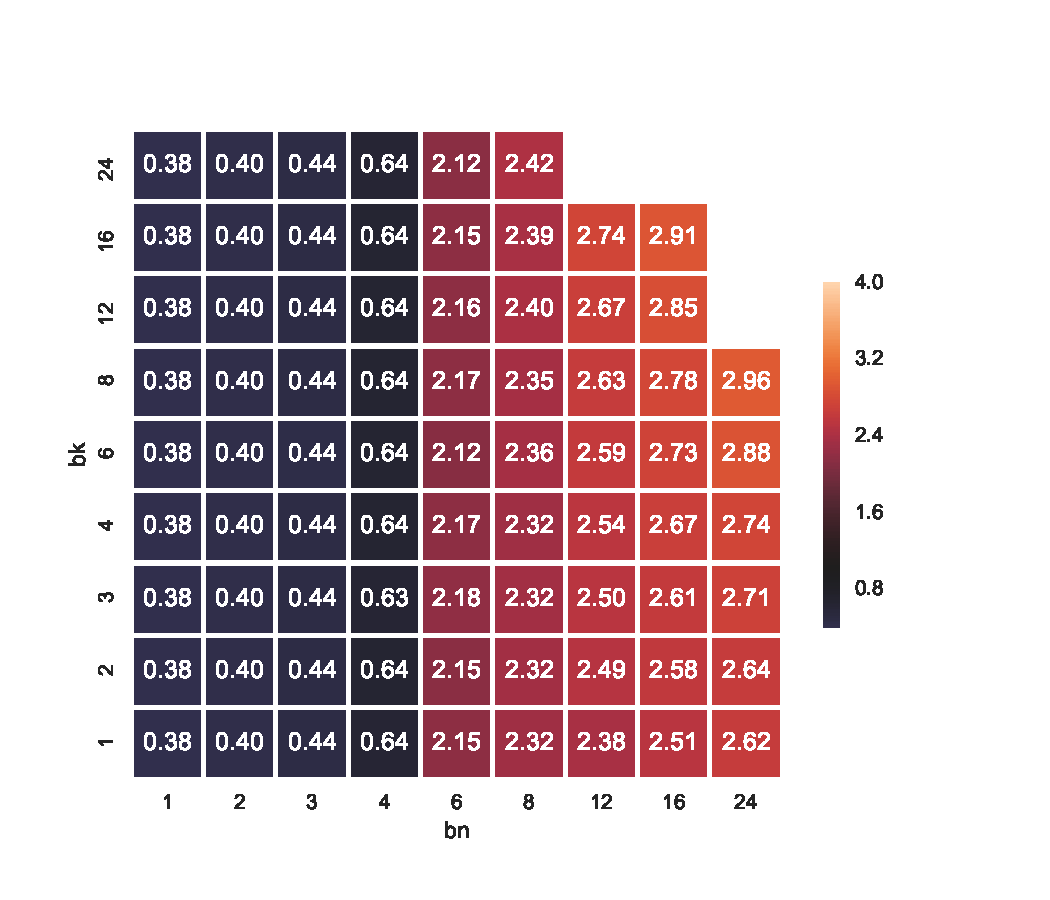
\includegraphics[width=\textwidth]{images/unrolled_sizing_2000_8.pdf}
      \caption{bm = 8, nnz = 2000}
    \end{subfigure}
    \begin{subfigure}[b]{0.45\textwidth}
      \centering
      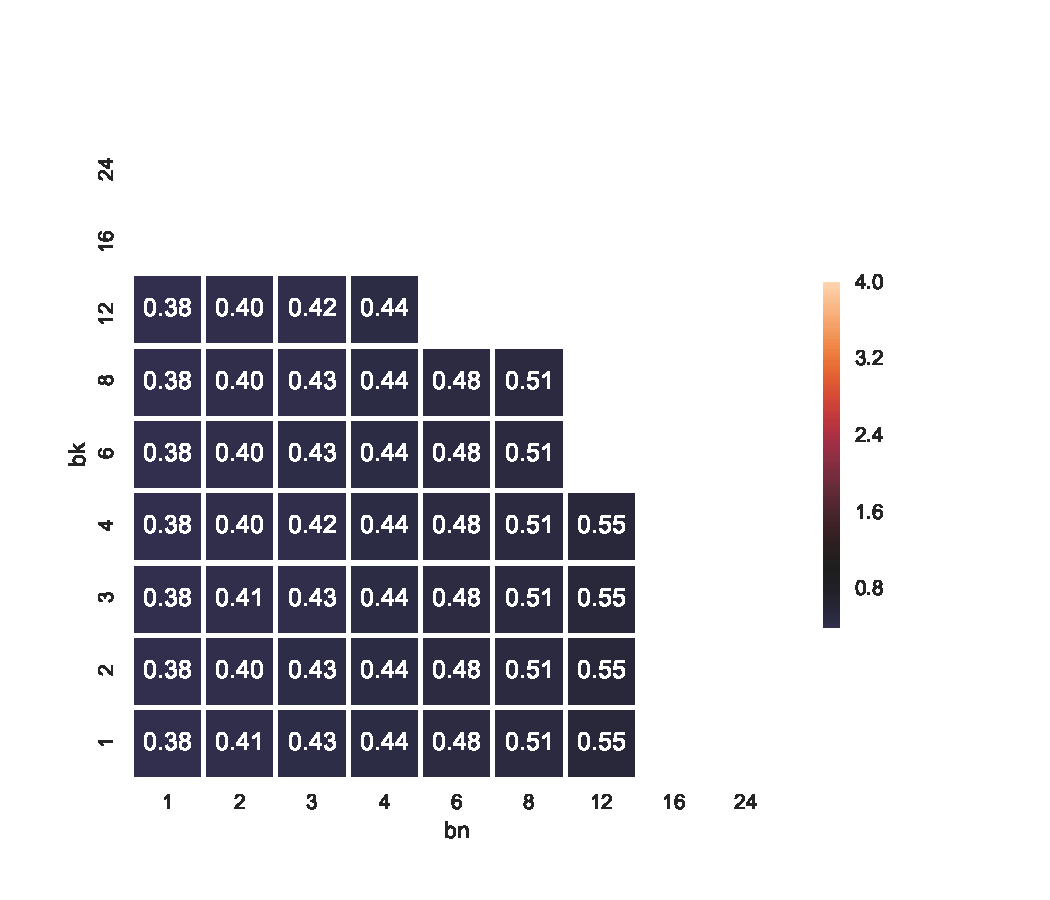
\includegraphics[width=\textwidth]{images/unrolled_sizing_2000_16.pdf}
      \caption{bm = 16, nnz = 2000}
    \end{subfigure}
    \caption{Effect of different block size choices}
    \label{fig:unrolled_sizing}
  \end{figure}


\section{Scaling of UnrolledSparse}

  Matrix sizes: $m=128, n=28, k=128$.
  Microkernel block sizes: $bm=8, bn=28, bk=4$.
  B is gradually filled with randomly placed nonzeros.

  \begin{figure}[!htb]
  	\centering
    \begin{subfigure}[b]{0.8\textwidth}
      \centering
      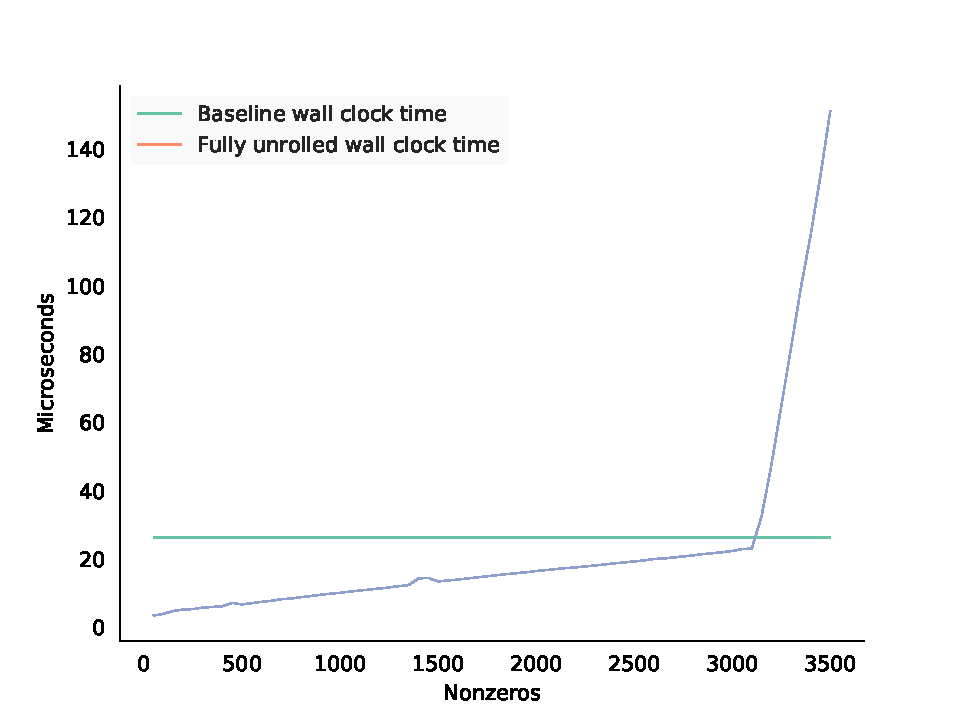
\includegraphics[width=\textwidth]{images/fig2.pdf}
      \caption{Time to solution for unrolledsparse}
      \label{fig:unrolled_time}
    \end{subfigure}
    \begin{subfigure}[b]{0.8\textwidth}
      \centering
      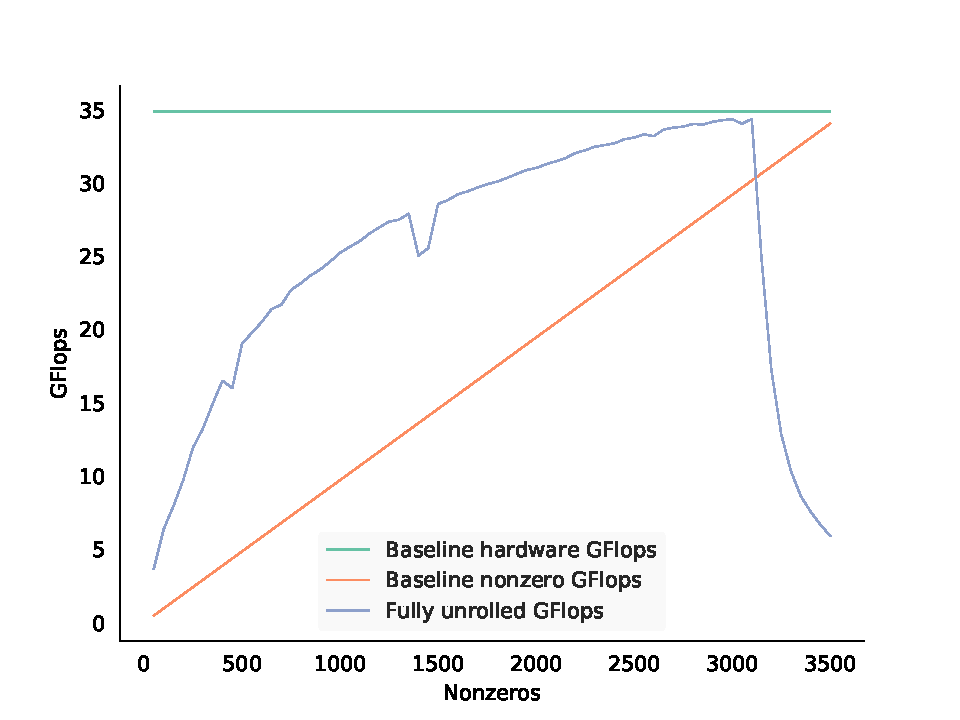
\includegraphics[width=\textwidth]{images/fig3.pdf}
      \caption{Performance of unrolledsparse}
      \label{fig:unrolled_perf}
    \end{subfigure}
  \end{figure}

  \begin{itemize}
    \item For $nnz < 3100$, time-to-solution scales linearly.
    \item For $nnz > 3200$, the FMAs completely fill the instruction cache (regardless of matrix dimensions!)
    \item Fully unrolled sparse algorithm outperforms dense ``nonzero'' GFlops, but always underperforms dense ``hardware'' GFlops
    

    Linear relationship between nnzs and time, with a constant offset compared to dense.

  \end{itemize} 


\section{Performance of GeneralSparse}

  \begin{figure}[!htb]
    \centering
    \begin{subfigure}[b]{0.8\textwidth}
      \centering
      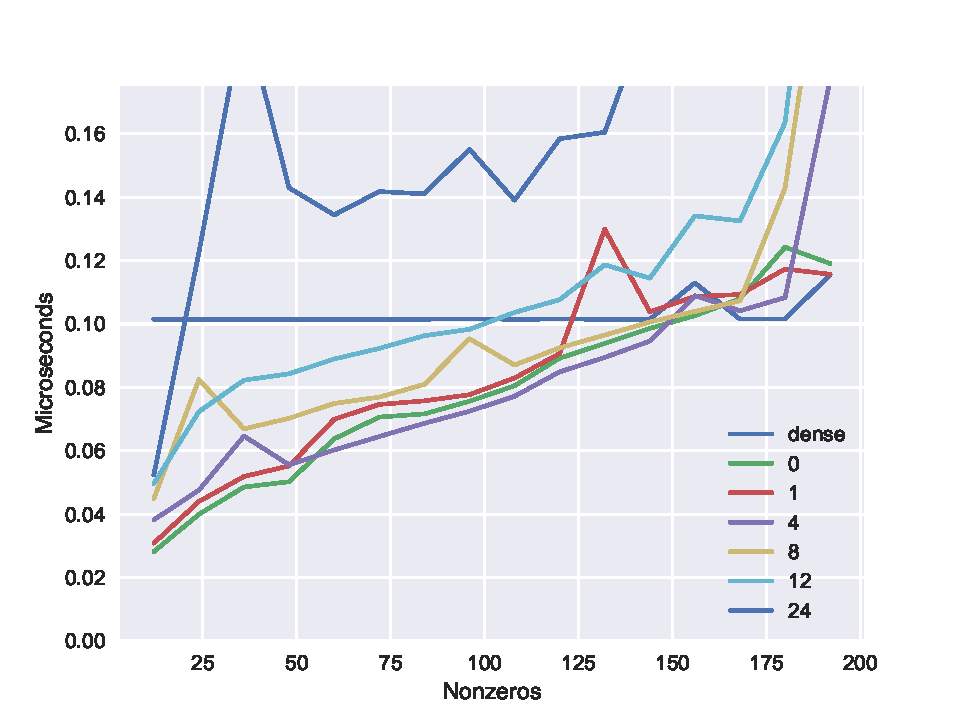
\includegraphics[width=\textwidth]{images/jump_penalty.pdf}
      \caption{Small-scale }
      \label{fig:unrolled_time}
    \end{subfigure}
    \begin{subfigure}[b]{0.8\textwidth}
      \centering
      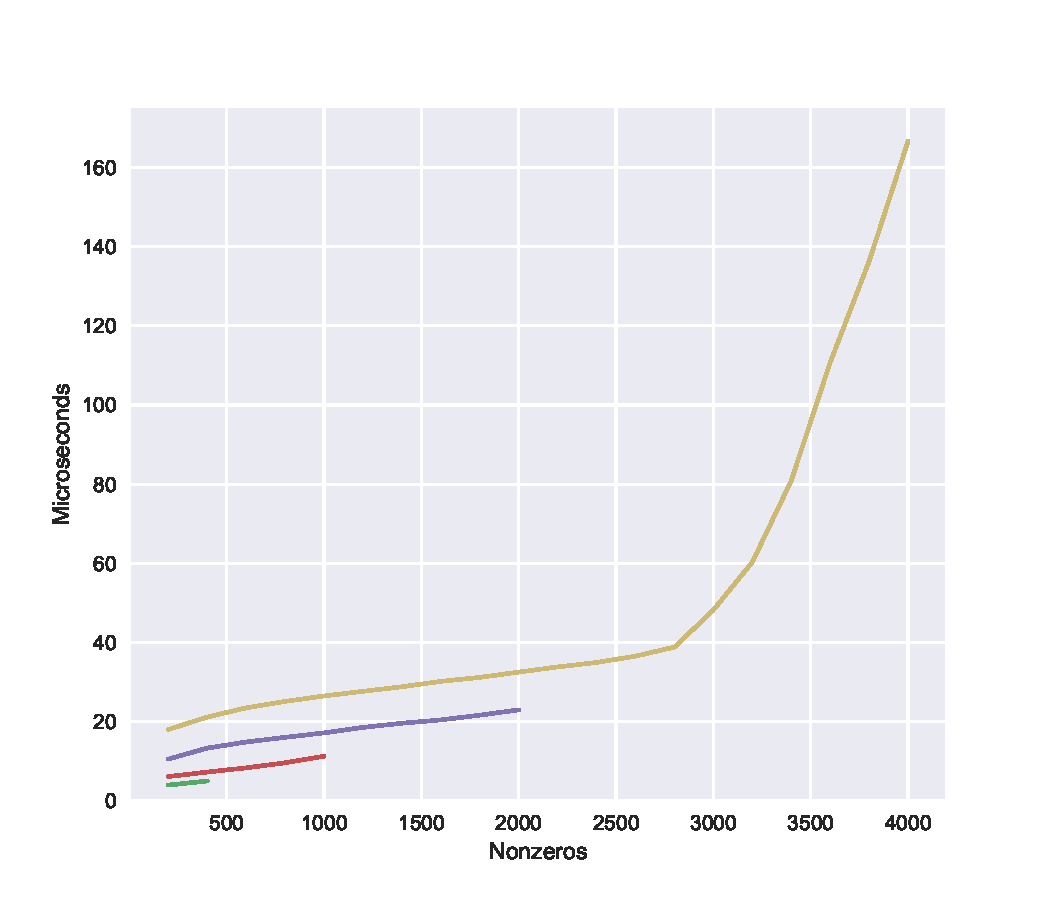
\includegraphics[width=\textwidth]{images/jump_scaling.pdf}
      \caption{Large-scale performance}
      \label{fig:unrolled_perf}
    \end{subfigure}
  \end{figure}


\section{Tensor multiplication}





 
\chapter{Conclusion}
\label{chapter:conclusion}


\section{Outlook}



 \clearemptydoublepage

 %\printglossaries

 \addcontentsline{toc}{chapter}{Bibliography}
 \bibliography{literature}
% % !TEX root = ../main.tex
\chapter{Detailed Descriptions}
%\section{Detailed Validation Results}
\label{chapter:DetailedDescriptions}\label{appendix}
%\inputminted{c++}{../../src/wos_native.cuh}
\newpage


\end{document}
